\part{Usage Examples}

\chapter{Citation}

\section{Traveling Salesman Problem}
旅行商问题(Traveling Salesman Problem, TSP)是组合优化领域的经典问题之一,其核心目标是给定城市列表和每对城市之间的距离,求恰好访问每个城市一次并返回起始城市的最短可能路线。该问题于1930年正式提出,是优化中研究最深入的问题之一,被用作许多优化方法的基准。自从该问题被正式提出以来,一直是运筹学、计算机科学和物流管理等领域的研究热点,尽管该问题在计算上很困难,但许多启发式方法和精确算法是已知的\cite{2009A, 2012Models}。

\begin{figure}[!htb]
    \centering
    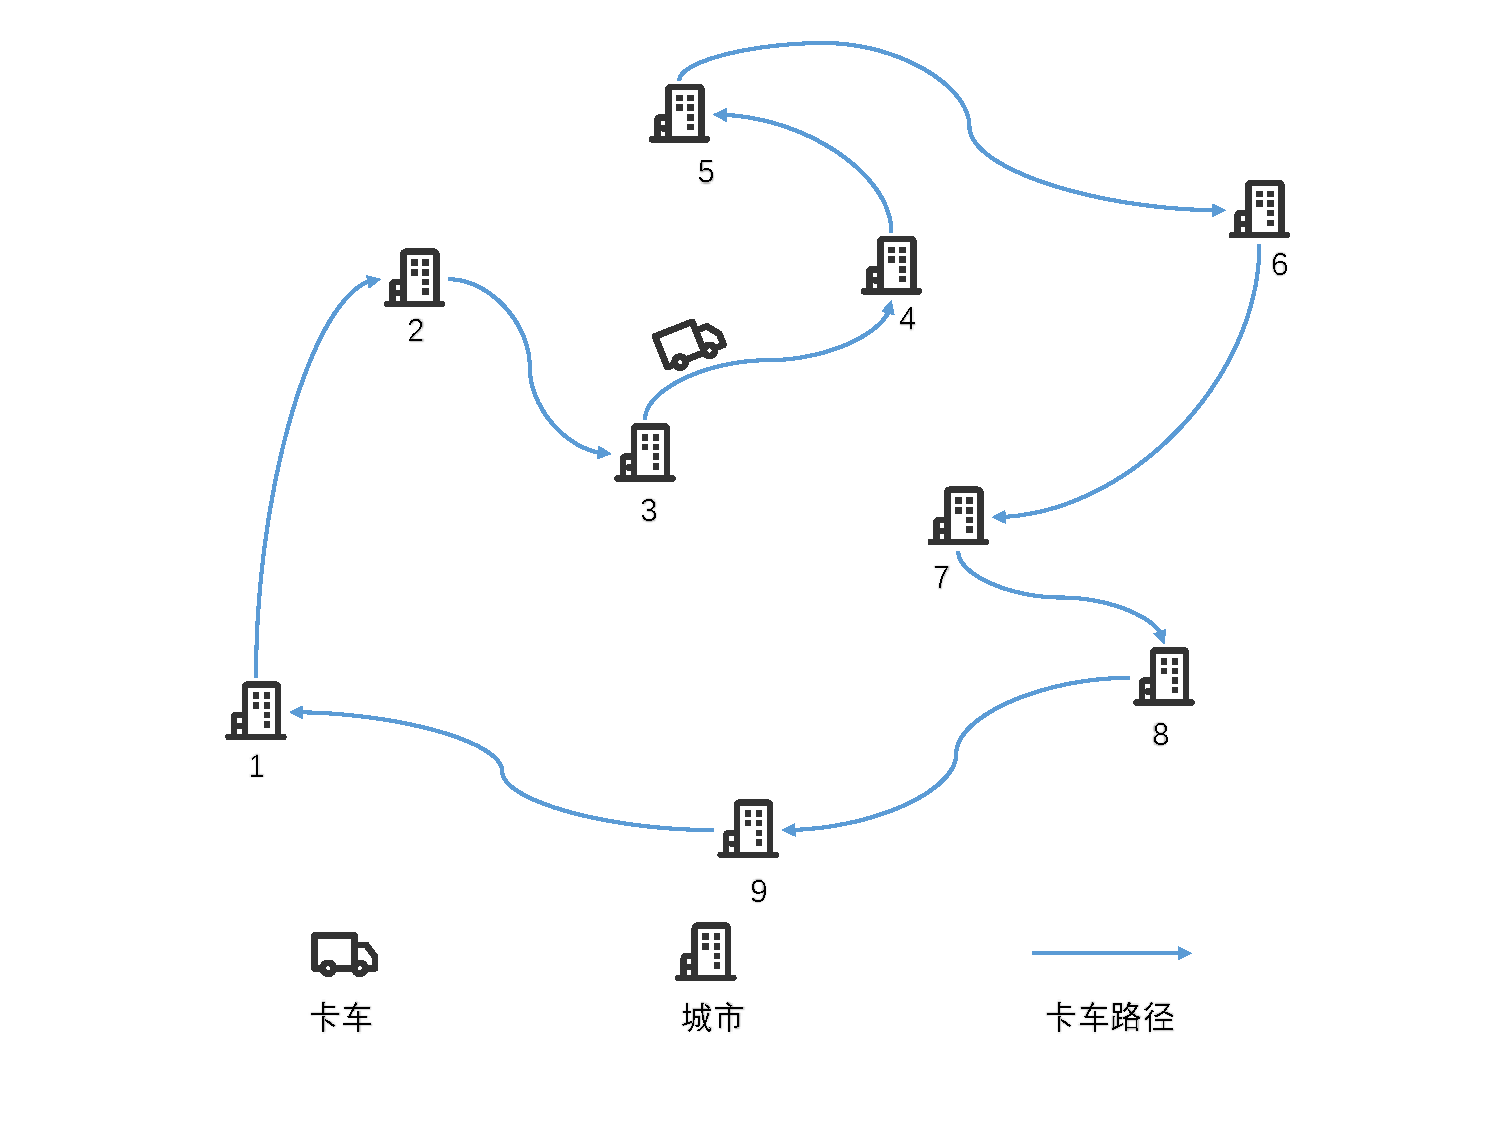
\includegraphics[width=\linewidth]{images/TSP.pdf}\\
    \caption{TSP示意图}
\end{figure}

TSP可以表述为整数线性规划模型\cite{papadimitriou1998combinatorial}:假设共有$N$个城市,每个城市的编号为$1,\cdots,N$,从城市$i$到城市$j$的旅行成本(距离)为$c_{ij}>0$。旅行商的目标是从任意一个城市出发访问完所有的城市,每个城市只能访问一次,最后回到最初的城市,目标是找到一条依次访问所有城市且访问城市不重复的最短路线。TSP中的决策变量为$x_{ij}=\begin{cases}1, & \text{存在从城市$i$到城市$j$的路径}\\0, & \text{其他} \end{cases}$,城市节点集合表示为$V(|V| = N)$。由于可能存在子回路,所以在构建TSP模型时需要消除会产生子回路的情况,这里采用Miller-Tucker-Zemlin(MTZ)约束进行子回路的消除\cite{1960Integer},引入连续变量$u_i(\forall i \in V, u_i \geq 0)$,其取值可以为任何非负实数(实数集合表示为$R$)。这里用$u_i$表示编号为$i$的城市的访问次序,比如当$u_i = 5$时表示编号为1的城市是从出发点开始,第5个被访问到的点。因此,TSP的数学模型可以表示为:

\begin{align}
    \min \quad & \sum_{i \in V}\sum_{j \in V, i \neq j} c_{ij}x_{ij} & \label{eq:tsp-obj}\\
    \text{s.t.} \quad & \sum_{i \in V} x_{ij} = 1, & \forall j \in V, i \neq j\label{eq:tsp-in}\\
    \quad & \sum_{j \in V} x_{ij} = 1, & \forall i \in V, i \neq j \label{eq:tsp-out}\\
    \quad & u_i - u_j + Nx_{ij} \leq N - 1, & \forall i, j \in V; i \neq j \label{eq:tsp-subtour}\\
    \quad & u_i \geq 0, & u_i \in R \label{eq:tsp-u_bound}\\
    \quad & x_{ij} \in \{0, 1\}, & i, j \in V; i \neq j\label{eq:tsp-x_bound}
\end{align}

目标函数\ref{eq:tsp-obj}表示最小化访问所有城市的成本(距离),约束\ref{eq:tsp-in}和\ref{eq:tsp-out}保证每个城市节点的入度和出度为1,即每个城市只进入一次和出去一次,保证了每个城市只访问一次,不会被重复访问,约束\ref{eq:tsp-subtour}消除子回路,约束\ref{eq:tsp-u_bound}和\ref{eq:tsp-x_bound}表示变量的取值范围。

\chapter{Formula}

\section{Flying Sidekick Traveling Salesman Problem}
Flying Sidekick Traveling Salesman Problem (FSTSP) 由Murray(2015)等\cite{murrayFlyingSidekickTraveling2015}提出。FSTSP数学模型的符号含义如表\ref{tab:fstsp-sign-meaning}所示。

\begin{table}[!htbp]
    \centering
    \caption{FSTSP模型符号及含义}
    \label{tab:fstsp-sign-meaning}
    \begin{tabularx}{\textwidth}{lX}
        \toprule[1pt] % 表头线宽1镑(point, pt)
        符号 & 含义 \\
        \midrule[0.75pt] % 表中间线宽0.75镑(point, pt)
        $0$ & 起点车场 \\
        $c + 1$ & 终点车场 \\
        $\mathbf{C}=\{1,2,\cdots,c\}$ & 全部客户集合 \\
        $\mathbf{C}' \subseteq \mathbf{C}$ & 无人机可访问的客户集合 \\
        $N_0 = \{0,1,2,\cdots,c\}$ & 流出节点集合 \\
        $N_+ = \{1,2,\cdots,c + 1\}$ & 流入节点集合 \\
        $N = \{0,1,2,\cdots,c,c + 1\}$ & 全部节点集合 \\
        $\langle i,j,k\rangle \in P, i \in N_0, j \in \mathbf{C}', j \neq i, k \in N_+, k \neq i, k \neq j$ & 无人机飞行路径集合(符合模型约束的路径) \\
        $\tau_{ij}'/\tau_{ij}$ & 弧$(i,j)$的飞行/行驶时间成本 \\
        $S_L/S_R$ & 无人机发射/回收耗时 \\
        $e$ & 无人机续航时长 \\
        $x_{ij} \in \{0,1\}$ & 卡车路由决策变量 \\
        $y_{ijk} \in \{0,1\}$ & 无人机路由决策变量 \\
        $1 \leq u_i \leq c + 2$ & 卡车破子圈辅助变量 \\
        $t_i'/t_i$ & 无人机/卡车有效到达时间戳辅助变量 \\
        $p_{ij} \in \{0,1\}$ & 无人机架次先后辅助变量 \\
        \bottomrule[1pt] % 表尾线宽1镑(point, pt)
    \end{tabularx}
\end{table}

FSTSP数学模型(部分)如下:
\definecolor{constraint-bg}{rgb}{0.9,0.9,1} % 定义浅蓝色背景

\begin{align}
    \min \quad & t_{c + 1}  \label{eq:fstsp-obj}\\
    \text{s.t.} \quad & \colorbox{constraint-bg}{$\displaystyle
      \sum_{\substack{i\in N_{0}\\i\neq j}}x_{ij} + 
      \sum_{\substack{i\in N_{0}\\ i\neq j}}
      \sum_{\substack{k \in N_{+}\\ \langle i,j,k \rangle \in P}}y_{ijk} = 1, \quad \forall j \in C 
    $} \label{eq:fstsp-customer-visit} \\
    \quad & \colorbox{yellow!30}{$\displaystyle
      \sum_{j\in N_{+}}x_{0j} = 1, \quad \text{(卡车出发约束)}
    $} \label{eq:fstsp-truck-start} \\
    \quad & \sum_{i\in N_{0}}x_{i,c + 1} = 1 \label{eq:fstsp-truck-return} \\
    \quad & \colorbox{green!30}{$\displaystyle
      u_i - u_j + 1 \leq (c + 2)(1 - x_{ij}), \quad \forall i \in C, j \in \{N_{+}:j \neq i\}
    $} \label{eq:fstsp-truck-mtz}
\end{align}

也可以如下表示:

\begin{align}
    \min \quad & t_{c + 1}  \label{eq:fstsp-obj}\\
    \text{s.t.} \quad & \colorbox{constraint-bg}{$\displaystyle\sum_{\substack{i\in N_{0}\\i\neq j}}x_{ij}+\sum_{\substack{i\in N_{0}\\ i\neq j}}\sum_{\substack{k \in N_{+}\\ \langle i,j,k \rangle \in P}}y_{ijk}=1$}, \quad \forall j \in C \label{eq:fstsp-customer-visit}\\
    \quad & \colorbox{yellow!30}{$\displaystyle\sum_{j\in N_{+}}x_{0j}=1$} \label{eq:fstsp-truck-start}\\
    \quad & \sum_{i\in N_{0}}x_{i,c + 1}=1 \label{eq:fstsp-truck-return}\\
    \quad & \colorbox{green!30}{$\displaystyle u_i - u_j + 1 \leq (c + 2)(1 - x_{ij})$}, \quad \forall i \in C, j \in \{N_{+}:j \neq i\} \label{eq:fstsp-truck-mtz}
\end{align}
